% Misión 6: la caza del objetivo. Portada y vuelo paso a paso.
% NED (este, norte): el anillo vial tiene centro E 0, N 42 y radio 26.5 m; la camioneta (ArUco 7) da vueltas
% antihorario a 3 m/s. Señuelos: ArUco 3 en E -38 N 36, 12 en E 36 N 40, 25 en E -12 N 79.
% Carriles del barrido: este -37.5, -12.5, 12.5, 37.5, de norte 0 a 78, a 15 m de altura.

\begin{frame}{Misión 6: la caza del objetivo}
  \begin{columns}[c]
    \column{0.56\textwidth}
    \begin{tikzpicture}
      \node[inner sep=0] (im) {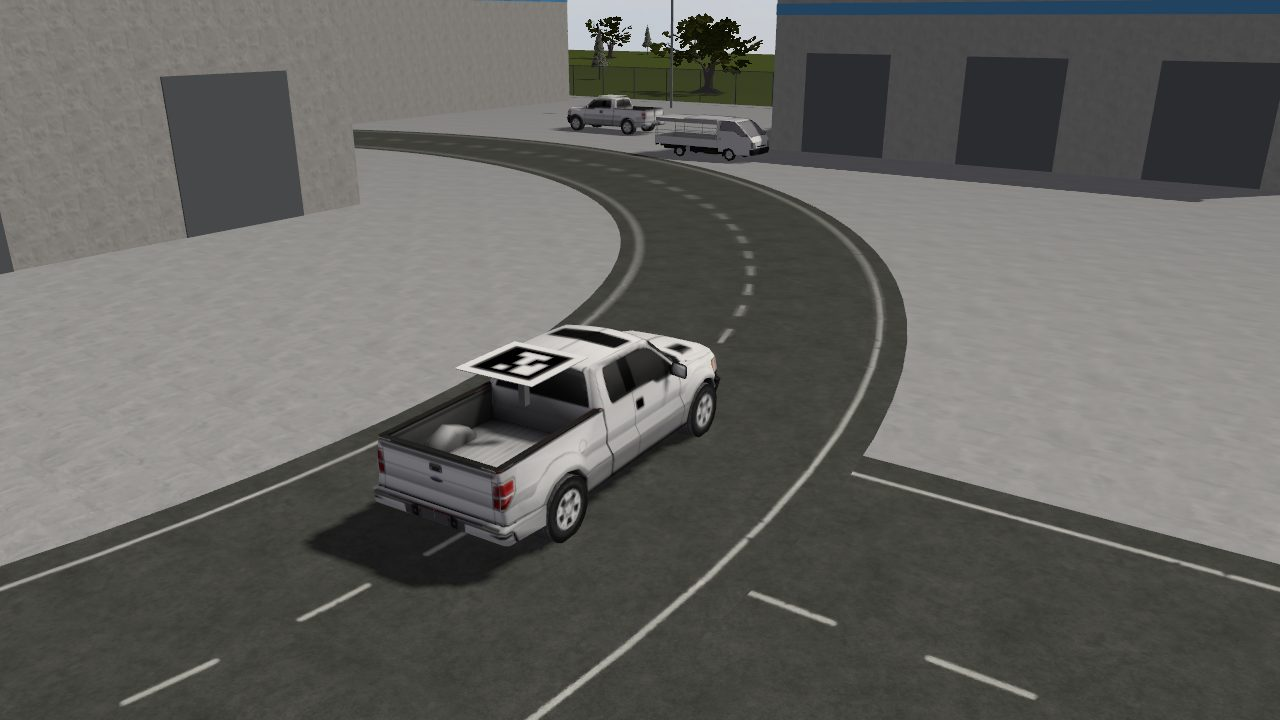
\includegraphics[width=\linewidth]{zona_bodegas_camioneta}};
      \node[anchor=north west,fill=azul,text=white,font=\bfseries\scriptsize,rounded corners=2pt]
        at ([xshift=4pt,yshift=-4pt]im.north west) {MISIÓN 6 · NIVEL 3 \nivel{3}};
    \end{tikzpicture}\\[0.3em]
    \small\textbf{Escenario}: una camioneta sospechosa da vueltas en una zona de bodegas. Hay que
    \textbf{encontrarla}, reconocerla por el \textbf{ArUco 7} de su techo (no los señuelos), dar su ubicación
    GPS y \textbf{seguirla} desde arriba.
    \column{0.41\textwidth}
    \ficha{x500_cam_abajo}{x500\_cam\_abajo}{zona\_bodegas}{caza\_objetivo + detector\_aruco}%
      {\cmd{square\_mission} y \cmd{velocity\_control}}{cámara, ArUco y perseguir algo que se \textbf{mueve}}%
      {60 s siguiéndola: a la vista $\geq$ 80 \%, distancia promedio \textless 1.5 m}
  \end{columns}
\end{frame}

\begin{frame}{La caza, paso a paso}
  \begin{columns}[c]
    \column{0.46\textwidth}\centering
    \begin{tikzpicture}[x=0.05cm,y=0.05cm]
      \draw[gray!50,fill=gray!8] (-55,-12) rectangle (55,85);
      \draw[gray!45,line width=5pt] (0,42) circle (26.5);
      \foreach \e in {-37.5,-12.5,12.5,37.5} \draw[azul!25,dashed] (\e,0) -- (\e,78);
      \node[draw,circle,fill=azulclaro,inner sep=0.3pt,font=\tiny] at (0,0) {H};
      % los señuelos
      \foreach \e/\n/\i in {-38/36/3,36/40/12,-12/79/25} {
        \fill[gray!70] (\e-2.5,\n-1.5) rectangle (\e+2.5,\n+1.5); \node[font=\tiny,text=gris,below] at (\e,\n-1.5) {\i};}
      % la camioneta (ángulo phi desde el este, antihorario)
      \foreach \s/\p in {1/270,2/330,3/118,4/150,5/200} {
        \only<\s>{\fill[rojo] ({26.5*cos(\p)-2.5},{42+26.5*sin(\p)-1.5}) rectangle ++(5,3);
                  \node[font=\tiny\bfseries,text=rojo] at ({26.5*cos(\p)},{42+26.5*sin(\p)+4}) {7};}}
      % lo que ve la cámara (36 m de ancho a 15 m) y el dron
      \only<1>{\fill[azul,opacity=0.12] (-55.5,-3.5) rectangle (-19.5,23.5); \node at (-37.5,10) {\dronarriba{0.6cm}};}
      \only<2>{\fill[azul,opacity=0.12] (-55.5,22.5) rectangle (-19.5,49.5); \node at (-37.5,36) {\dronarriba{0.6cm}};}
      \only<3>{\fill[azul,opacity=0.12] (-30.5,51.5) rectangle (5.5,78.5); \node at (-12.5,65) {\dronarriba{0.6cm}};}
      \only<4>{\node at ({26.5*cos(150)},{42+26.5*sin(150)}) {\dronarriba{0.6cm}};
        \draw[-{Stealth},naranja,thick] ({26.5*cos(150)},{42+26.5*sin(150)}) -- ++({-0.5*12},{-0.866*12});}
      \only<5>{\node at ({26.5*cos(185)},{42+26.5*sin(185)}) {\dronarriba{0.6cm}};
        \draw[naranja,dashed,thick,-{Stealth}] ({26.5*cos(186)},{42+26.5*sin(186)}) arc (186:198:26.5);}
      \only<6>{\node at (0,0) {\dronarriba{0.6cm}};}
      \draw[azul,thick,-{Stealth},visible on=<1-2>] (-37.5,0) -- (-37.5,78);
      \draw[azul,thick,-{Stealth},visible on=<3>] (-37.5,0) -- (-37.5,78) -- (-12.5,78) -- (-12.5,66);
    \end{tikzpicture}
    \column{0.52\textwidth}
    \estados{1-2/SEARCH,3-4/FOLLOW,5/LOST,6/RETURN}
    \vspace{0.3em}

    \only<1>{\begin{terminal}{ros2 launch x500\_retos caza.launch.py}
caza\_objetivo: buscando el ArUco 7\\
Arriba. Barriendo el patio
    \end{terminal}\small A 15 m la cámara ve \textasciitilde36\,$\times$\,27 m ({\color{azul}azul}). Barre el patio en
      carriles norte--sur, como una podadora.}%
    \only<2>{\begin{terminal}{caza\_objetivo}
Veo el ArUco 3: es un señuelo, lo ignoro
    \end{terminal}\small Un coche estacionado con ArUco. \textbf{No es el 7}: lo anuncia una vez y sigue.}%
    \only<3>{\begin{terminal}{caza\_objetivo}
Veo el ArUco 25: es un señuelo, lo ignoro\\
¡OBJETIVO ENCONTRADO! ArUco 7 en NED\\
\ \ norte 65.4, este -12.4 (lat ..., lon ...)\\
Siguiéndolo durante 60 s
    \end{terminal}\small Del píxel a metros (con la actitud del dron) y de metros a GPS.}%
    \only<4>{\begin{terminal}{caza\_objetivo}
siguiendo: a 0.8 m, va a 3.0 m/s (20 s)
    \end{terminal}\small \textbf{Tus TODO}: estimar su velocidad y apuntar a donde \textbf{va a estar}
      ({\color{naranja}flecha}), no a donde la viste.}%
    \only<5>{\begin{terminal}{caza\_objetivo}
Lo perdí de vista hace 3.0 s: voy a donde\\
\ \ debería estar\\
¡Lo recuperé!
    \end{terminal}\small Si la pierde, sigue la predicción. Si en 8 s no aparece, vuelve al barrido.}%
    \only<6>{\begin{terminal}{caza\_objetivo}
Fin del seguimiento. Regresando a casa\\
objetivo encontrado: sí\\
a la vista: 93 \% del seguimiento (mínimo 80) OK\\
distancia promedio: 0.84 m (máximo 1.5) OK
    \end{terminal}\credito{Números de ejemplo: dependen de tus TODO y de dónde iba la camioneta.}}%
  \end{columns}
\end{frame}
